\documentclass{beamer}
\usepackage[english,french]{layout}
\usepackage[utf8]{inputenc}
\usepackage[english]{babel}
\usepackage[T1]{fontenc}
\usepackage{lmodern}
\usepackage{textcomp}

\usepackage{graphicx} %The mode "LaTeX => PDF" allows the following formats: .jpg  .png  .pdf  .mps
\usepackage{animate}
\usepackage{amsmath, soul, color, multicol, type1cm, verbatim, latexsym, dsfont, float, listings,alltt}
\usepackage[official]{eurosym}
\usepackage{beamerthemesplit}
\usetheme{Frankfurt}
\usefonttheme{professionalfonts}
\setbeamercovered{transparent}
%NeSI Colors <-------------------------------------------------------------------------------------
\usecolortheme{lily}
\usecolortheme[RGB={47, 68, 71}]{structure} 
\definecolor{nesidark}{HTML}{2F4447}
\definecolor{nesilight}{HTML}{CED9DF}
\definecolor{nesigrey}{gray}{0.7}
\definecolor{nesilightgrey}{gray}{0.98}
\definecolor{nesidarkgrey}{gray}{0.3}
\definecolor{nesiblue}{HTML}{2B9FC2}

\setbeamertemplate{headline}{}

\setbeamercolor{block title}{fg=black,bg=nesigrey}
\setbeamercolor{block body}{bg=nesilightgrey,fg=nesidarkgrey}
\setbeamercolor{block body alerted}{bg=white,fg=black}
\setbeamercolor{alerted text}{bg=white,fg=black}
%NeSI Title <---------------------------------------------------------------------------------------
\setbeamerfont{title}{size=\huge}
\frenchspacing
\hyphenation{NeSI}
%NeSI Template parameters <-------------------------------------------------------------------------
\setbeamertemplate{blocks}[default]
\useinnertheme{circles}
\setbeamertemplate{title page}[default][center,rounded=false,shadow=false]
\newcommand\BackgroundPicture[1]{%
\setbeamertemplate{background}{%
\parbox[c][\paperheight]{\paperwidth}{%
\vfill \hfill \includegraphics[height=0.9\paperheight]{#1}
\hfill \vfill
}}}

%Content Starts Here <-------------------------------------------------------------------------------
\title[Permeability simulations]{Meso- and macro scale permeability simulations on the
Pan cluster}
%\subtitle{Computational Science team}
\author{Bart Verleye, Elinor Swery, Piaras Kelly}
\date{}

\begin{document}

{
\setbeamertemplate{background canvas}{
\includegraphics[height=0.99\paperheight]{NeSI_img/Slide00.png}} 
\begin{frame}[plain]
\vspace{1cm}
\titlepage
\end{frame}
}




%%%%%%%%%%%%%%%%%%%%%%%%%%%%%%%%%%%%%%%%%%%%%%%%%%%%%%%%%%%%%%%%%%%%%%%%%%%%%%%%%%%%%%%%%%%%%%%
%%%%%%%%%%%%%%%%%%%%%%%%%%%%%%%%%%%%%%%% Some Examples %%%%%%%%%%%%%%%%%%%%%%%%%%%%%%%%%%%%%%%%%%%
%%%%%%%%%%%%%%%%%%%%%%%%%%%%%%%%%%%%%%%%%%%%%%%%%%%%%%%%%%%%%%%%%%%%%%%%%%%%%%%%%%%%%%%%%%%%%%%
\frame[t]
{
\frametitle{Introduction: Composite material}
\begin{figure}
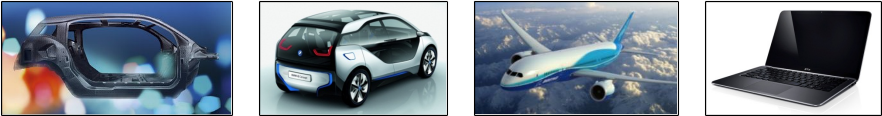
\includegraphics[width=\textwidth]{_img/Usage}
\end{figure}
\begin{block}{ Composite material}
Two or more constituent materials with significantly different physical or chemical properties, 
that when combined to produce a material with characteristics different from the individual components: 
\begin{enumerate}
 \item Reinforcement e.g.\ carbon fiber;
 \item Matrix e.g.\ hardened resin. 
\end{enumerate}

 \end{block}

}

\frame[t]{
\frametitle{Production process}
\begin{block}{Liquid Composite Moulding}
\begin{figure}
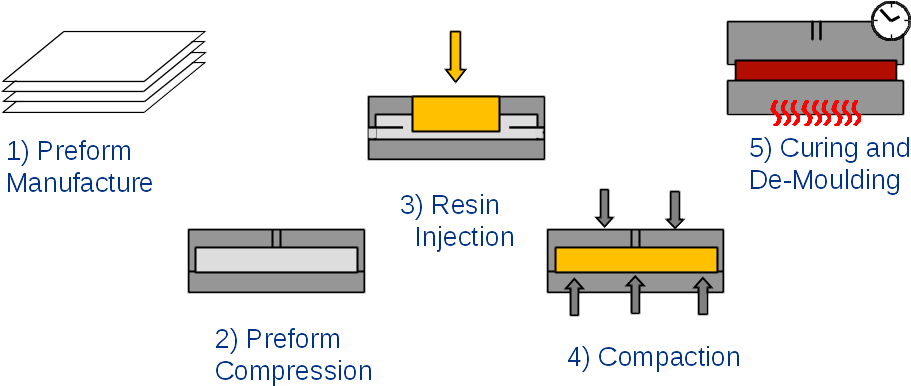
\includegraphics[width=\textwidth]{_img/LCM}
\end{figure}
\end{block}
}

\frame[t]{
\frametitle{Production process: Simulation}

\animategraphics[autoplay,loop,height=2.5cm]{5}{videos/png_files/Pictures}{1}{202} 
\animategraphics[autoplay,loop,height=2.5cm]{5}{videos/png_files/Pressure}{1}{202}

\begin{block}{Outputs of simulations are used to optimise the process by selecting:}
\begin{itemize}
 \item Injection times
 \item  Injection locations
 \item  Vent locations
 \item Injection pressures
 \item Press size
 \item Energy consumption
\end{itemize}
\end{block}
}

\frame[t,shrink=20]{
\frametitle{Permeability}
\begin{block}{Definition}
Permeability characterises the ease with which a fluid can flow through
the reinforcement
\end{block}

\begin{block}{Permeability depends on:}
\begin{columns}[c]
 \column{.45\textwidth}
\begin{itemize}
 \item Fibre volume fraction
 \item Compaction applied
 \item Stitching
\end{itemize}
 \column{.55\textwidth}
\begin{itemize}
 
 \item Reinforcement architecture
 \item Laminate structure and nesting
 \item Geometric variability
\end{itemize}
\end{columns}
\end{block}

\begin{columns}[t,onlytextwidth]
\column{.45\textwidth}
\begin{block}{Textile Modelling:}
  \begin{itemize}
   \item Automatic
    \item Repeatable
    \item Complex fibre architecture
     \item Computationally Intensive
    \item Requires validation
   \end{itemize}
\end{block}
 \column{.45\textwidth}
 \begin{block}{Experiments:}
 \begin{itemize}
      \item Complex fibre architecture
      \item Capture nesting
      \item Time consuming – User intensive
      \item Difficult to perform accurately
     \end{itemize}
     \end{block}
\end{columns}
}

\frame[t,shrink=10]{
\frametitle{Meso vs. Macro scale}
\begin{block}{
MACRO}
\begin{figure}
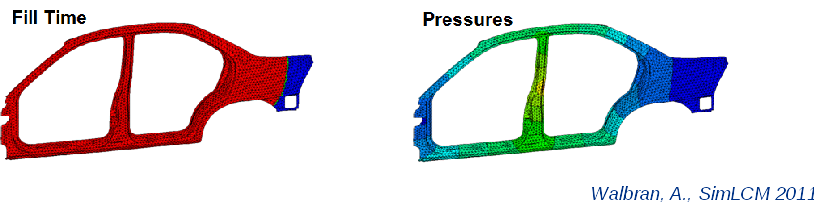
\includegraphics[width=\textwidth]{_img/Output}
\end{figure}
\end{block}
\begin{block}{
MESO}
\begin{figure}
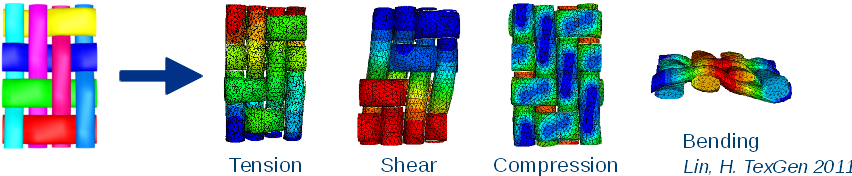
\includegraphics[scale=0.5]{_img/Deformation}
\end{figure}
\end{block}
}

\frame[t,shrink=10]{
\frametitle{Macro scale}
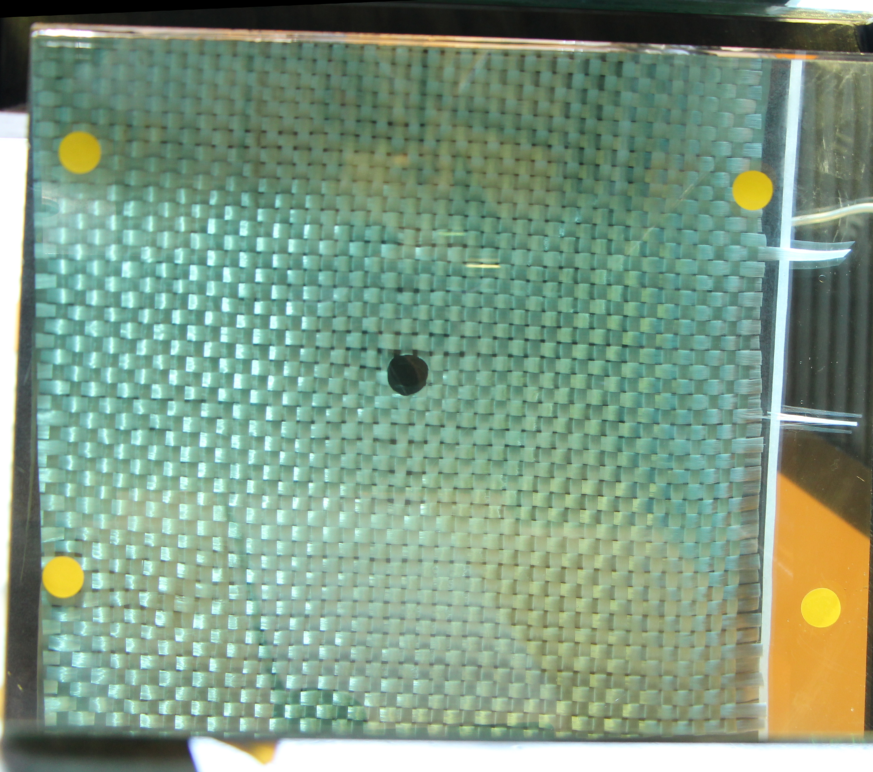
\includegraphics[width=0.4\textwidth]{_img/textile}
\includegraphics[width=0.4\textwidth]{_img/TextileModel2.jpg}

}


\frame[t]{
\frametitle{Meso and Macro}
\begin{itemize}
 \item A full CFD simulation on a macro-scale model is almost impossible and would take too much resources.
 \item Solution: (many) Meso-scale simulations that provide input for an easier macro-simulation. 
 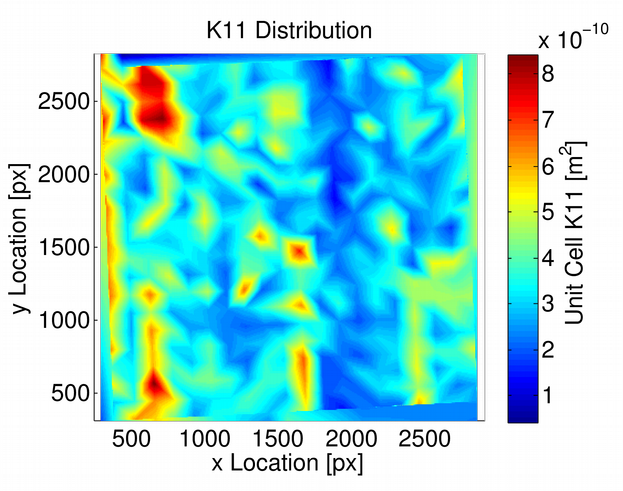
\includegraphics[scale=0.45]{_img/PermeabilityMap}\\
\end{itemize}

}


\frame[t]{
\frametitle{6 different programs }
%\begin{figure}
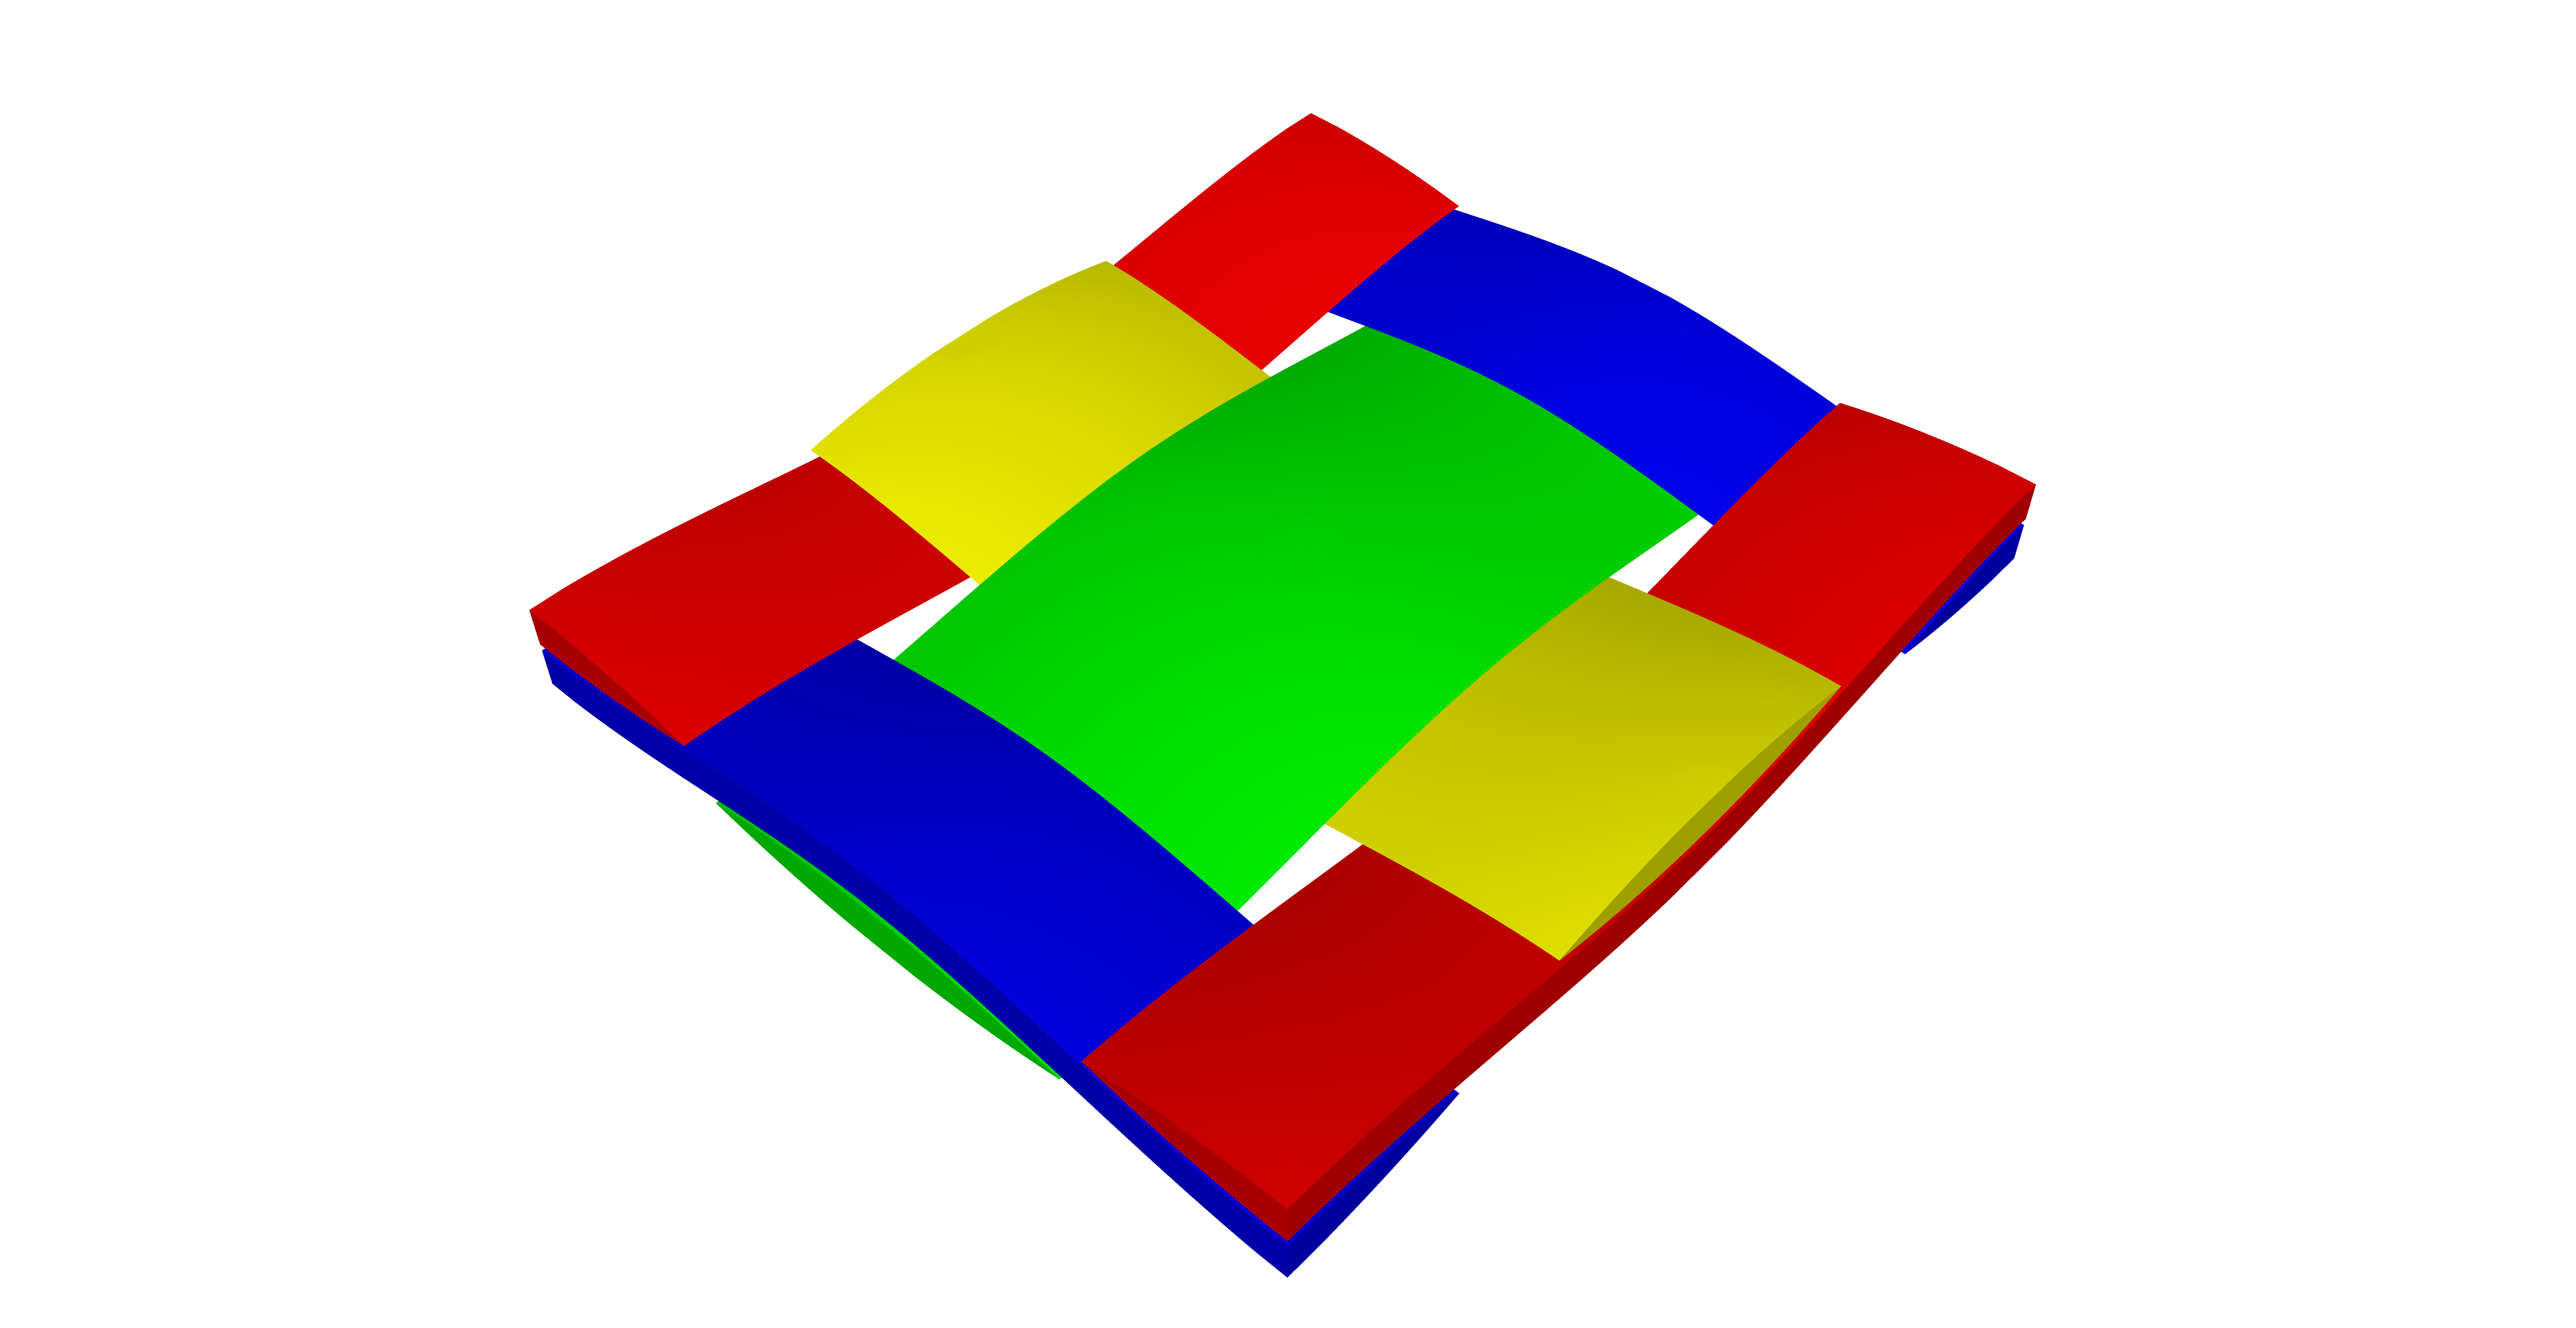
\includegraphics[width=0.3\textwidth]{_img/tg3}
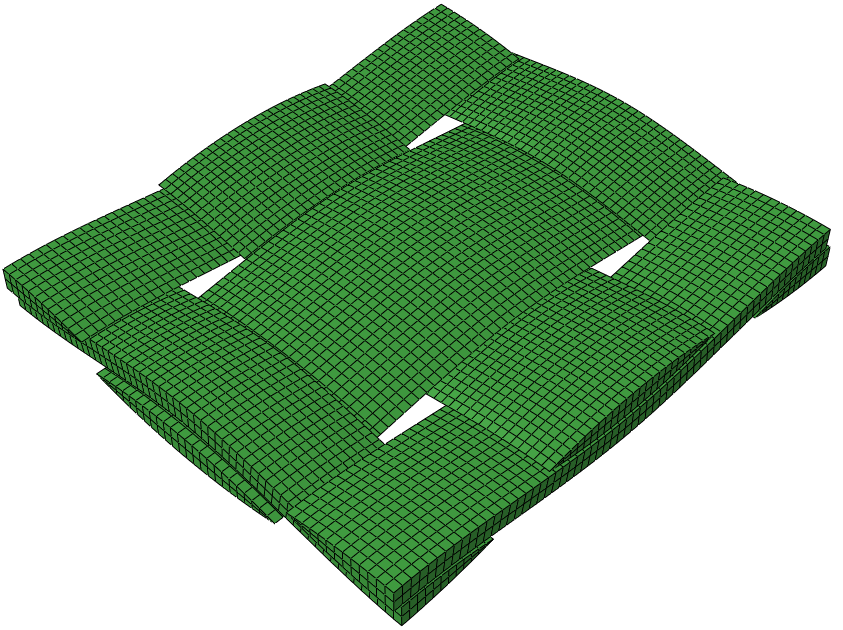
\includegraphics[width=0.3\textwidth]{_img/abaqusMesh}
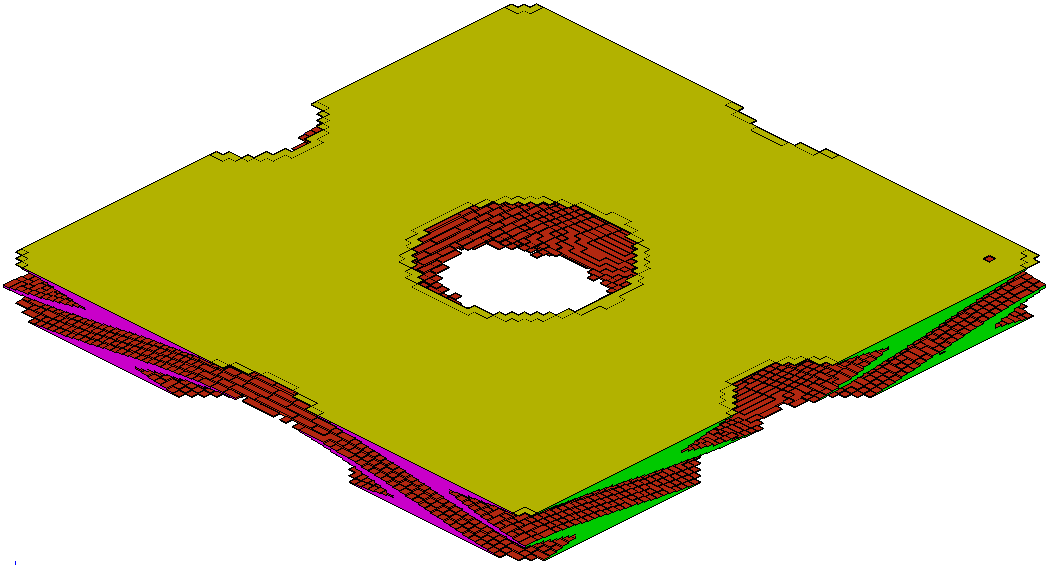
\includegraphics[width=0.3\textwidth]{_img/hypermesh}\\
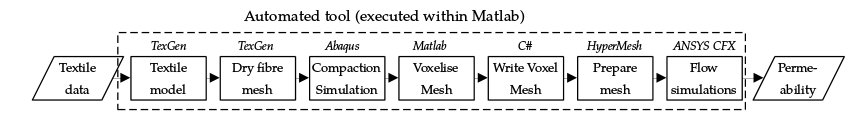
\includegraphics[width=\textwidth]{_img/BR-3}\\
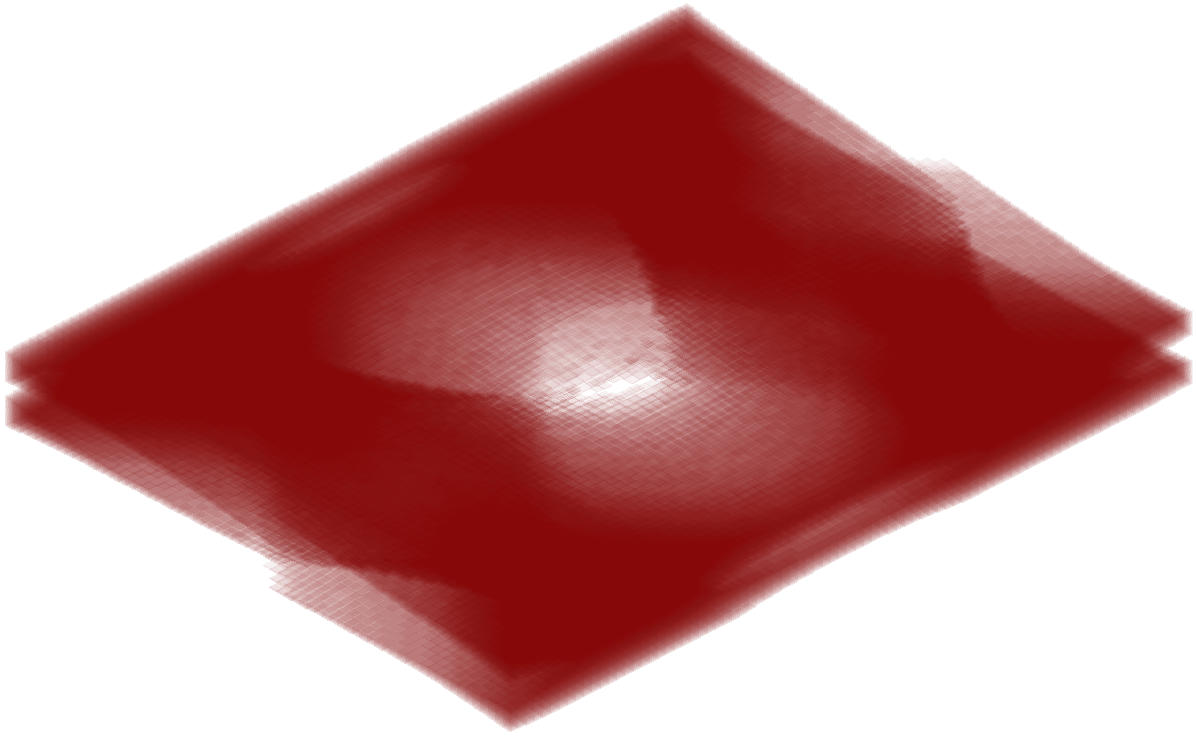
\includegraphics[width=0.3\textwidth]{_img/mesh3}
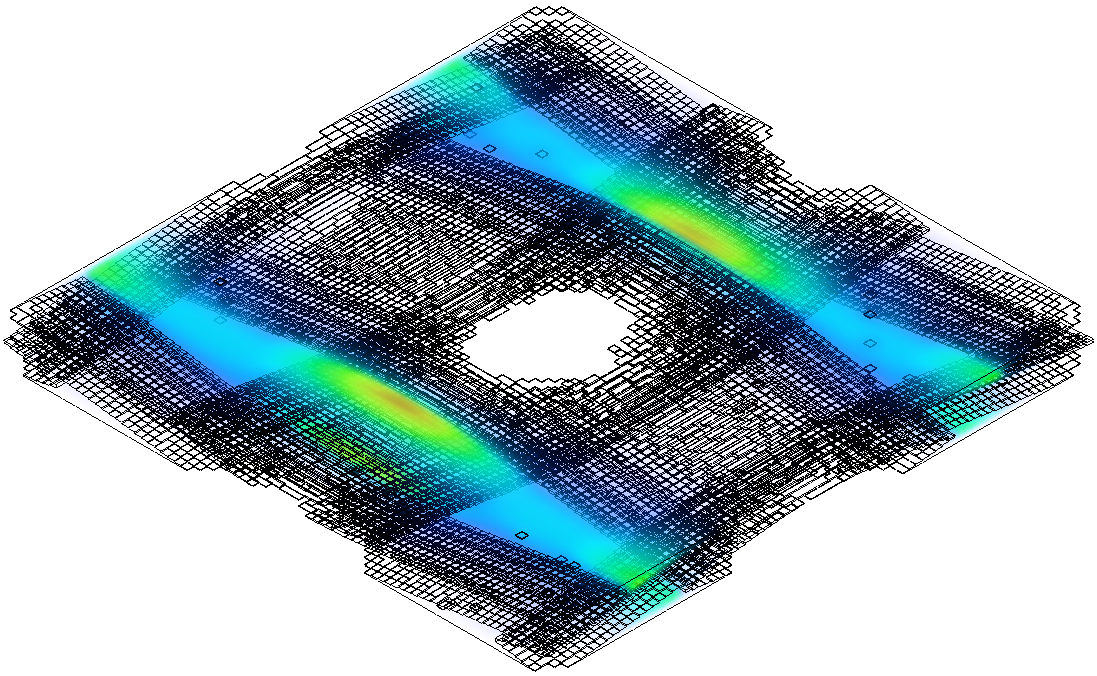
\includegraphics[width=0.3\textwidth]{_img/ansysvelocity}
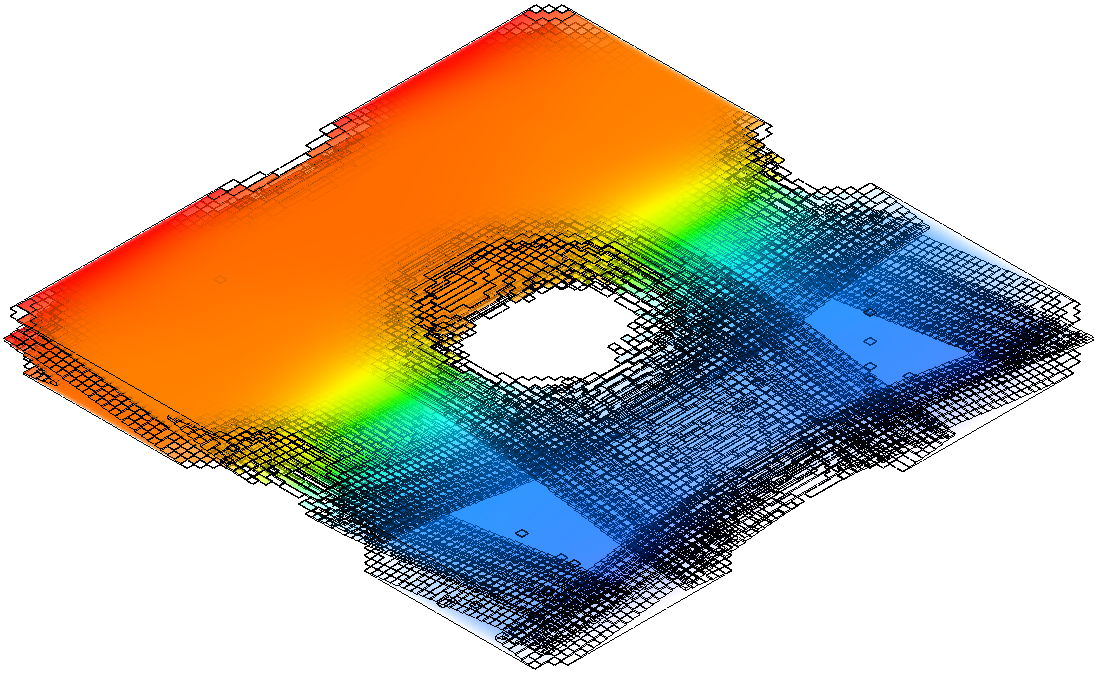
\includegraphics[width=0.3\textwidth]{_img/ansyspressure}
%\end{figure}
}

\frame[t]{
\frametitle{6 different programs }
\begin{figure}
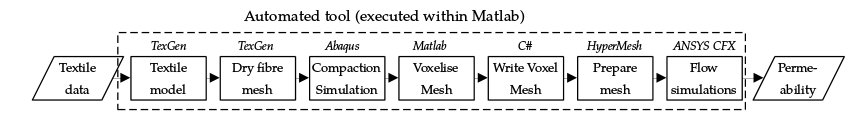
\includegraphics[scale=0.5]{_img/BR-3}
\end{figure}
To make the tool work on Pan, following steps were undertaken:
\begin{enumerate}
 \item Install TexGen and compile the C\# software. Abaqus, Matlab, ANSYS and
Hypermesh are available modules on Pan.
 \item Define the correct command lines for all the software. In case of
HyperMesh, this was only able to be completed with help from the
supplier.
 \item Adapt the scripts and input files for a Linux system, including changing
hard coded paths.
 \item Split up the main script and provide a Slurm scheduler input file for every
step. This is important for the macro-scale simulation (see further).
 \item Write a script that submits all Slurm files as a chain job.
\end{enumerate}
}

\frame[t]{
\frametitle{6 different programs }
\begin{figure}
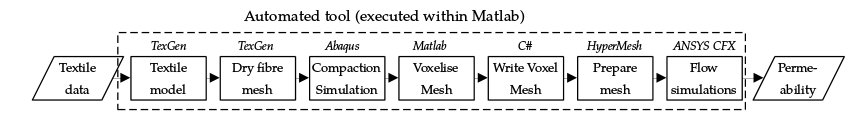
\includegraphics[scale=0.5]{_img/BR-3}
\end{figure}
\begin{block}{
The different steps have different requirements:}
\begin{itemize}
 \item TexGen, Hypermesh and C\# only run serial.
 \item Abaqus and ANSYS can run parallel.
 \item Solution: 6 different SLURM jobs with dependencies. 
\end{itemize}
\end{block}
}
\frame[t]{
\frametitle{Experiment}
\begin{figure}
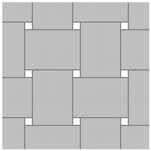
\includegraphics[width=0.2\textwidth]{_img/2D-model}
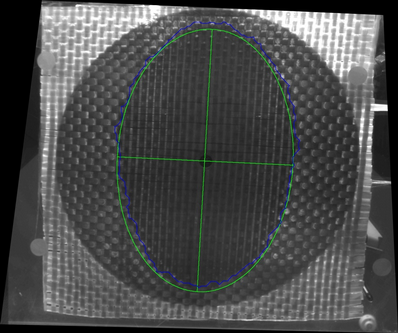
\includegraphics[width=0.3\textwidth]{_img/experiment}
\end{figure}
\begin{block}{
2D in plance single layer}
\begin{itemize}
 \item Different thicknesses: 1.2, 0.9, 0.7\,mm
 \item Different volume fractions:0.25, 0.34, 0.47\,\%
\end{itemize}
\end{block}
}
\frame[t]{
\frametitle{Results}
\begin{figure}
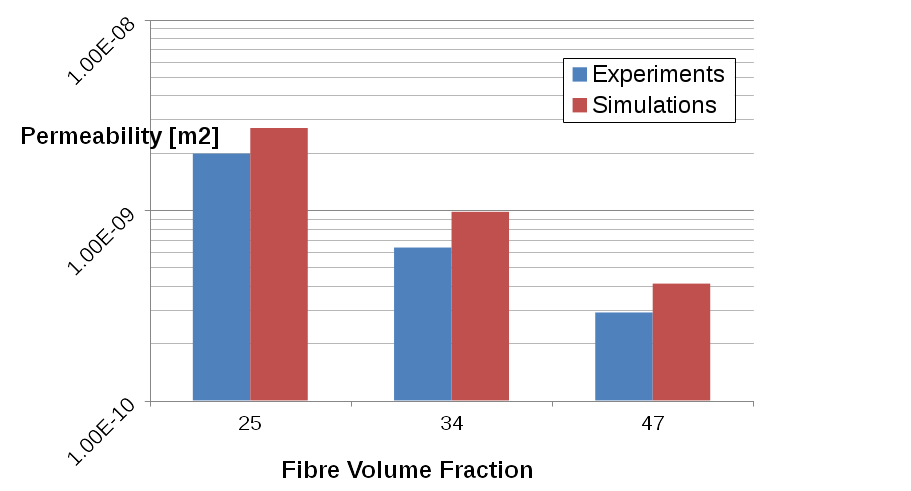
\includegraphics[width=\textwidth]{_img/results}
\end{figure}
}

{
\setbeamertemplate{background canvas}{
\includegraphics[height=0.99\paperheight]{NeSI_img/Slide00.png}} 
\begin{frame}[plain]
\begin{center}
{\Huge Questions \& Answers}
\end{center}
\end{frame}
}


\end{document} 
